\documentclass[border=5pt]{standalone}
\usepackage{tikz}
\usepackage{amsmath}
\begin{document}
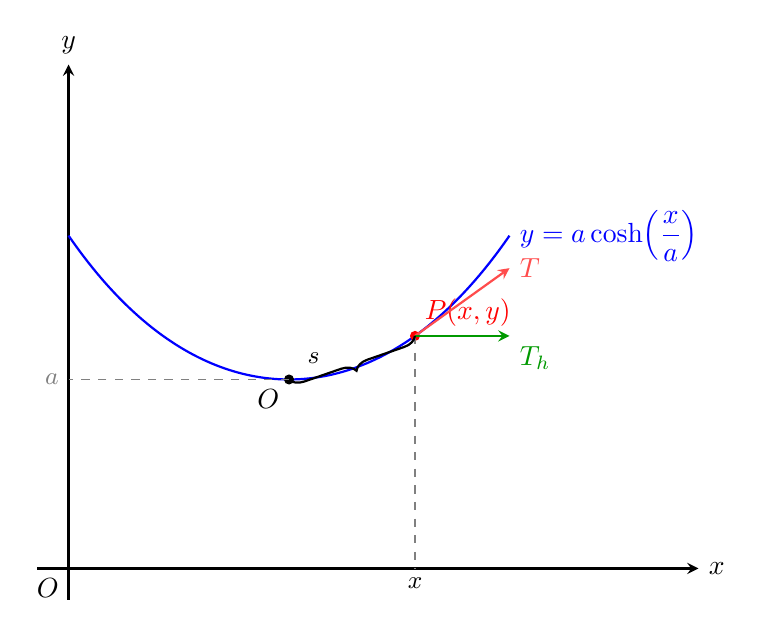
\begin{tikzpicture}[scale=0.8, >=stealth]
  % Coordinate axes
  \draw[->, thick] (-0.5,0) -- (10,0) node[right] {$x$};
  \draw[->, thick] (0,-0.5) -- (0,8) node[above] {$y$};

  % Catenary curve y = 3*cosh(x/3)
  \draw[blue, thick, domain=-3.5:3.5, samples=200]
    plot ({\x+3.5}, {3*cosh(\x/3)}) node[right] {$y = a\cosh\!\left(\dfrac{x}{a}\right)$};

  % Point P on curve
  \pgfmathsetmacro{\tx}{2}
  \pgfmathsetmacro{\px}{\tx+3.5}
  \pgfmathsetmacro{\py}{3*cosh(\tx/3)}
  \filldraw[red] (\px, \py) circle (2pt) node[above right] {$P(x,y)$};

  % Bottom of chain (origin of arc length)
  \filldraw[black] (3.5, 3) circle (2pt) node[below left] {$O$};

  % Tension vector at P (tangent to curve)
  \pgfmathsetmacro{\dydx}{sinh(\tx/3)}
  \draw[->, thick, red!70] (\px, \py) -- ++(1.5, {1.5*\dydx}) node[right] {$T$};

  % Horizontal tension component
  \draw[->, thick, green!60!black] (\px, \py) -- ++(1.5, 0) node[below right] {$T_h$};

  % Vertical line from P to x-axis showing weight
  \draw[dashed, gray, thin] (\px, \py) -- (\px, 0);
  \node[below, font=\small] at (\px, 0) {$x$};

  % Arc length s label
  \draw[decorate, decoration={brace, amplitude=5pt, mirror}, thick]
    (3.5, 3) -- (\px, \py) node[midway, left=8pt, font=\small] {$s$};

  % Origin label
  \node[below left] at (0,0) {$O$};

  % y-axis label for chain
  \draw[dashed, gray, thin] (3.5, 3) -- (0, 3) node[left, font=\small] {$a$};
\end{tikzpicture}
\end{document}
